\documentclass[aps,pra,twocolumn,superscriptaddress,nofootinbib]{revtex4-2}
\usepackage{amsmath,amssymb,graphicx,booktabs,hyperref}

\begin{document}

\title{Evidence-conditioned correlated matching for surface codes under circuit-level noise}

\author{evmatch authors}
\date{\today}

\begin{abstract}
Matching decoders turn each error mechanism of a circuit-level detector error
model into graph edges and give every edge the mechanism's full probability,
even when the syndrome rules the mechanism out. We show that a local,
syndrome-dependent correction to the edge weights closes the gap between
correlated minimum-weight perfect matching and belief-matching. The rule is that a multi-edge mechanism contributes
probability to its edges only if each of its edges touches a detection event.
It costs $O(\#\text{detection events})$ per shot, and we combine it with the
standard two-pass correlated reweighting. For the rotated surface-code memory
under SI1000 noise at distances 5, 7 and 9 and physical error rates
0.2--0.5\%, the resulting decoder makes 7--17\% fewer logical errors than the
correlated mode of PyMatching~2. The advantage grows with distance. In paired
tests it is statistically indistinguishable from belief-matching at $d=5,7$
and better at $d=9$, while running at 4.6--7.2$\times$ the time of
uncorrelated PyMatching (1.7--2.2$\times$ its correlated mode). The decoder
is open source, sinter-compatible and built on PyMatching's sparse blossom.
\end{abstract}

\maketitle

\section{Introduction}

Minimum-weight perfect matching (MWPM) is the standard decoder for the
surface code, and sparse blossom~\cite{higgott2023sparse} makes it fast
enough for real-time use. MWPM is not optimal under circuit-level noise,
because many error mechanisms flip more than two detectors. A $Y$ error on a
data qubit, for example, flips both $X$-type and $Z$-type detectors. The
detector error model (DEM) decomposes such a mechanism into graph edges, and
the decoder then treats those edges as independent.

Correlated matching~\cite{fowler2013optimal} recovers part of the lost
information. It decodes once, lowers the weights of edges that share a
mechanism with the chosen edges, and decodes again. PyMatching ships this as
\texttt{enable\_correlations} since version 2.3. Belief-matching~\cite{higgott2023improved}
goes further: it sets the edge weights from belief-propagation (BP) marginals
over the full hypergraph, at roughly $10^3$ times the cost.

Correlated matching uses only \emph{positive} evidence: a mechanism becomes
more likely when one of its edges is matched. It never uses \emph{negative}
evidence, namely that a mechanism whose other part shows no syndrome
practically did not happen. Yet every edge in the matching graph carries the
full probability of every mechanism containing it. Paths through edges whose
correlated partners are silent therefore look cheaper than they are. This
paper isolates that effect and corrects it locally.

\section{Method}

\paragraph{Graph construction.}
We merge DEM instructions by symptom, the set of detectors flipped. Each
merged mechanism $h$ has probability $p_h$ and a decomposition $E(h)$ into
edges. Stim may decompose instructions with the same symptom differently: it
splits $Y$-type errors into $X$ and $Z$ parts even when the symptom is a
single edge. When every decomposition is applied separately, as PyMatching
does, probability leaks onto edges the mechanism never flips alone, often
boundary edges. We instead keep, for each symptom, the offered decomposition
with the fewest components. The edge prior is the independent (XOR)
combination
$q_e = \bigoplus_{h \ni e} p_h$.

\paragraph{Evidence gate.}
Let $D$ be the set of detection events. An edge $e=(u,v)$ is \emph{touched}
if $u \in D$ or $v \in D$. A multi-edge mechanism $h$ ($|E(h)|\ge2$) is
\emph{active} if every edge of $E(h)$ is touched. The per-shot edge
probability is
\begin{equation}
  q_e(D) = \Big(\bigoplus_{h \ni e,\ |E(h)|=1} p_h\Big) \oplus
           \Big(\bigoplus_{h \ni e,\ h\ \mathrm{active}} p_h\Big).
\end{equation}
An inactive multi-edge mechanism would have to occur together with a second
error that cancels its symptom exactly, a higher-order event, so it is
dropped. Active mechanisms are found by walking the edges incident to
detection events, so the gate costs $O(|D|)$.

\paragraph{Two passes.}
We match with weights $w_e = \log\frac{1-q_e(D)}{q_e(D)}$ and trace the
matched paths. Each edge $e_2$ that shares a mechanism with an edge $e_1$ on
those paths then gets $w_{e_2} \leftarrow \min(w_{e_2}, \log\frac{1-r}{r})$,
with $r = \min(\tfrac12, P(e_1 \wedge e_2)/P(e_1))$. This is PyMatching's
correlated rule, with joint probabilities precomputed from the DEM. We then
match again. All weight changes are written in place into the sparse-blossom
graphs and undone after the shot.

\section{Benchmark}

We use the rotated surface-code memory experiment (Z basis, $d$ rounds) from
Stim~\cite{gidney2021stim}. Each CX is compiled to H$\cdot$CZ$\cdot$H, and
we apply SI1000 noise~\cite{gidney2022benchmarking}: two-qubit depolarizing
$p$ after CZ, $p/10$ after single-qubit gates and on idle qubits, an extra
$2p$ on qubits idling during measurement or reset, $2p$ reset flips and $5p$
measurement flips. Logical error rates come from sinter with $10^6$ shots
per point. Differences between decoders are measured on identical shots
(paired), with McNemar's test on the discordant shots. Times are
single-threaded on the same pre-sampled shots.

\section{Results}

\begin{table}[t]
\caption{Paired comparison with correlated PyMatching (v2.4.0) on identical
shots. Ratio = evmatch errors / correlated errors, $\pm2\sigma$ from the
discordant shots. Time is relative to uncorrelated PyMatching.}
\label{tab:paired}
\begin{tabular}{rrrrrr}
\toprule
$d$ & $p$ & shots & ratio & McNemar $p$ & time \\
\midrule
5 & 0.3\% & 400k & $0.924\pm0.017$ & $5\times10^{-20}$ & 4.9$\times$ \\
5 & 0.5\% & 400k & $0.934\pm0.008$ & $2\times10^{-61}$ & 4.6$\times$ \\
7 & 0.3\% & 400k & $0.886\pm0.026$ & $9\times10^{-19}$ & 5.1$\times$ \\
7 & 0.5\% & 400k & $0.920\pm0.010$ & $4\times10^{-62}$ & 4.8$\times$ \\
9 & 0.2\% & 2M & $0.859\pm0.051$ & $3\times10^{-8}$ & 6.6$\times$ \\
9 & 0.3\% & 400k & $0.835\pm0.040$ & $2\times10^{-16}$ & 5.9$\times$ \\
9 & 0.5\% & 400k & $0.887\pm0.011$ & $5\times10^{-97}$ & 4.8$\times$ \\
\bottomrule
\end{tabular}
\end{table}

\begin{figure*}[t]
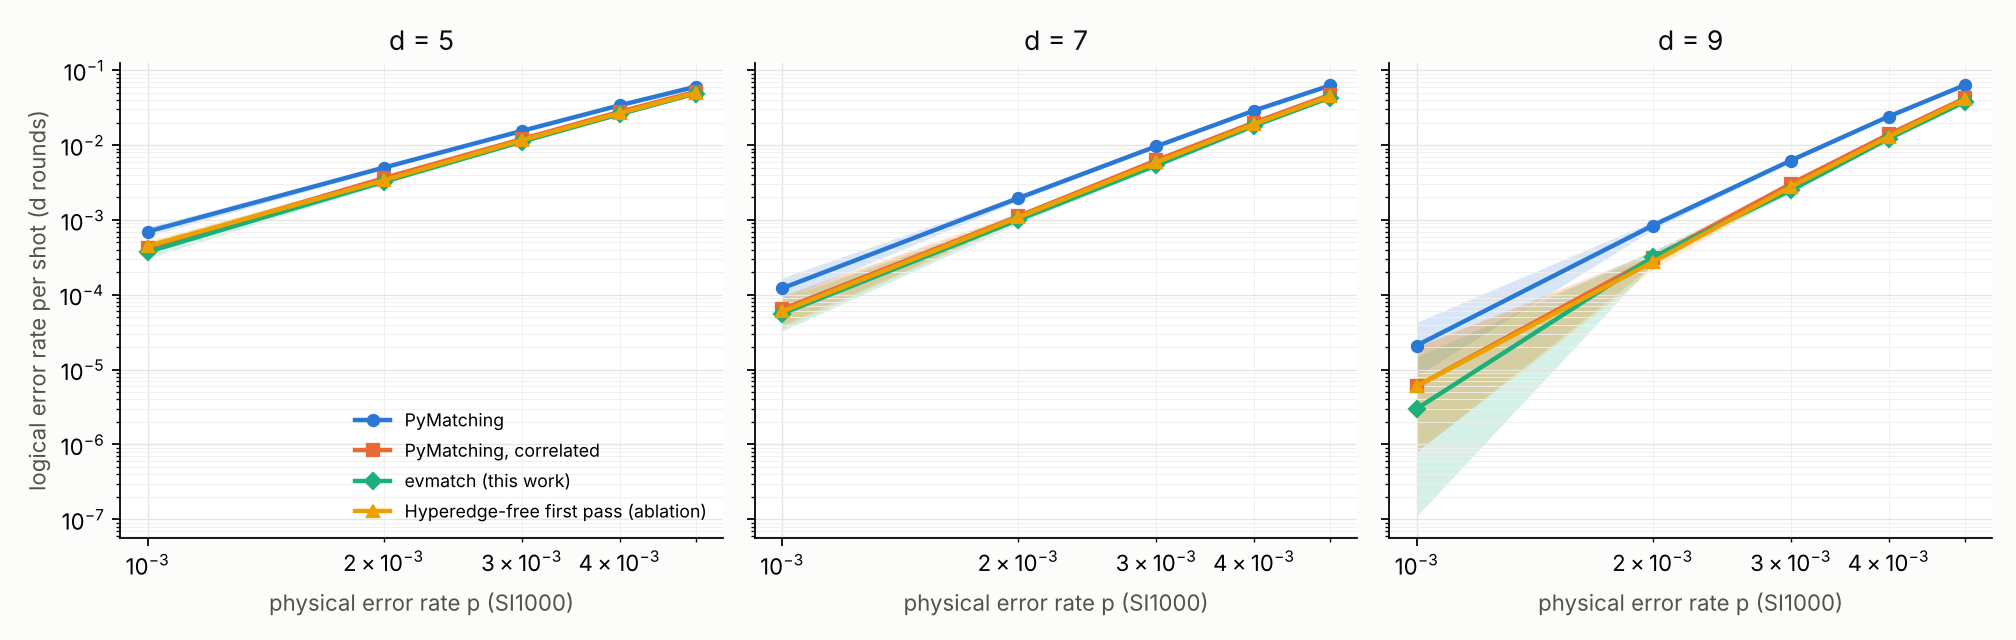
\includegraphics[width=\textwidth]{../results/ler.png}
\caption{Logical error rate per shot ($d$ rounds) under SI1000 noise,
$10^6$ shots per point (sinter); bands are likelihood intervals
(max-likelihood factor 1000).}
\label{fig:ler}
\end{figure*}

Table~\ref{tab:paired} and Fig.~\ref{fig:ler} summarize the results. The
reduction relative to correlated matching grows with distance, from 7\% at
$d=5$ to 11--17\% at $d=9$. Over the full grid,
$p\in\{0.1,\dots,0.5\}\%$, evmatch costs 4.6--7.2$\times$ uncorrelated
PyMatching; the worst case is $d=9$, $p=0.1\%$, where the fixed per-shot
costs of path tracing dominate.

\paragraph{Ablation.} Table~\ref{tab:ablation} separates the contributions
at $d=9$, $p=0.3\%$. The fewest-components decomposition alone gives 2\%.
Dropping hyperedges from the base graph without any evidence gate gives a
further 4\%; this is like the first pass of the correlated decoder inside
Harmony~\cite{shutty2024efficient}. The evidence gate contributes the
remaining 11\%. Applying the gate to the second pass only recovers most, but
not all, of that 11\%. Using the gate without the correlated pass is
\emph{worse} than correlated matching: the positive and the negative evidence
are complementary.

\begin{table}[t]
\caption{Ablation, paired, $d=9$, $p=0.3\%$, 400k shots.}
\label{tab:ablation}
\begin{tabular}{lr}
\toprule
decoder & errors \\
\midrule
PyMatching, correlated & 1210 \\
\quad + fewest-components decomposition & 1184 \\
\quad + hyperedge-free base graph, no gate & 1141 \\
\quad + evidence gate, second pass only & 1054 \\
\quad + evidence gate, both passes (evmatch) & 1010 \\
evidence gate, single pass, no correlations & 1965 \\
\bottomrule
\end{tabular}
\end{table}

\paragraph{Belief-matching.} Against the reference \texttt{beliefmatching}
package (20 BP iterations), on identical shots, the error counts were
1096 vs 1132 ($d=5$, $p=0.3\%$, $10^5$ shots) and 4761 vs 4696 ($p=0.5\%$),
and 290 vs 309 and 2148 vs 2180 at $d=7$ ($5\times10^4$ shots). None of these
differences is significant ($p>0.15$). At $d=9$, $p=0.3\%$, evmatch made 70
errors against 110 for belief-matching ($2.5\times10^4$ shots, $p=9\times10^{-6}$);
there the reference implementation was also worse than correlated matching.
% TODO: d=9 p=0.5% and the no-shortcut variant.

\section{Related work}

Positive-only correlated reweighting appears in Fowler's original
method~\cite{fowler2013optimal}, its pipelined version~\cite{paler2023pipelined},
PyMatching~2.3, Tesseract's multi-pass mode, and the alternating $X$/$Z$
schemes of Refs.~\cite{delfosse2014decoding,yuan2022modified}. Detection-event-driven
local reweighting also appears in Google's real-time decoder
(``preweight correlations'')~\cite{google2025below}, in Paler and Fowler's
virtual pre-matching~\cite{paler2023pipelined}, and in the split-fault rule of
Ref.~\cite{grans2023improved}. All of these only \emph{lower} weights. The DGR
decoder~\cite{wang2023dgr} also raises weights, but it conditions on a previous
matching, not on the syndrome, and learns correlations across shots.
Belief-matching~\cite{higgott2023improved} captures negative evidence through
global BP. Ensembles (Harmony~\cite{shutty2024efficient},
Libra~\cite{jones2024improved}), neural decoders~\cite{bausch2024learning}
and search-based decoders~\cite{beni2025tesseract} are more accurate but cost
orders of magnitude more or are not open. Decoder switching~\cite{toshio2025decoder}
sends only low-confidence shots to belief-matching and is complementary to
our approach.

\section{Discussion}

The evidence gate is a crude, local stand-in for the BP posterior: it keeps
the part of the conditioning that matters to a matching decoder, namely
whether a correlated partner is visible in the syndrome. It drops the part
that hurts matching, which is penalizing the interior of error chains whose
detectors fire twice. It needs nothing beyond the DEM, adds no parameters, and
fits into existing correlated-matching implementations as a different base
graph plus a per-shot restore step. Open questions include graded rather than
binary evidence, more than two passes, other codes (colour codes, where most
mechanisms are hyperedges), and hardware data.

\paragraph{Code and data.} \url{https://github.com/JimmyCarvalho/evmatch}
(Apache-2.0), including the circuits, all raw sinter statistics and the
scripts that produce every number in this paper.

\begin{thebibliography}{99}
\bibitem{higgott2023sparse} O.~Higgott and C.~Gidney, Sparse Blossom: correcting a million errors per core second with minimum-weight matching, Quantum \textbf{9}, 1600 (2025), arXiv:2303.15933.
\bibitem{fowler2013optimal} A.~G.~Fowler, Optimal complexity correction of correlated errors in the surface code, arXiv:1310.0863 (2013).
\bibitem{higgott2023improved} O.~Higgott, T.~C.~Bohdanowicz, A.~Kubica, S.~T.~Flammia and E.~T.~Campbell, Improved decoding of circuit noise and fragile boundaries of tailored surface codes, Phys. Rev. X \textbf{13}, 031007 (2023).
\bibitem{gidney2021stim} C.~Gidney, Stim: a fast stabilizer circuit simulator, Quantum \textbf{5}, 497 (2021).
\bibitem{gidney2022benchmarking} C.~Gidney, M.~Newman and M.~McEwen, Benchmarking the planar honeycomb code, Quantum \textbf{6}, 813 (2022).
\bibitem{shutty2024efficient} N.~Shutty, M.~Newman and B.~Villalonga, Efficient near-optimal decoding of the surface code through ensembling, arXiv:2401.12434 (2024).
\bibitem{paler2023pipelined} A.~Paler and A.~G.~Fowler, Pipelined correlated minimum weight perfect matching of the surface code, Quantum \textbf{7}, 1205 (2023).
\bibitem{delfosse2014decoding} N.~Delfosse and J.-P.~Tillich, A decoding algorithm for CSS codes using the X/Z correlations, arXiv:1401.6975 (2014).
\bibitem{yuan2022modified} Y.~Yuan and C.-C.~Lu, A modified MWPM decoding algorithm for quantum surface codes over depolarizing channels, arXiv:2202.11239 (2022).
\bibitem{google2025below} Google Quantum AI and collaborators, Quantum error correction below the surface code threshold, Nature \textbf{638}, 920 (2025).
\bibitem{grans2023improved} L.~Grans-Samuelsson \emph{et al.}, arXiv:2310.12981 (2023). % TODO verify title
\bibitem{wang2023dgr} Wang \emph{et al.}, arXiv:2311.16214 (2023). % TODO verify title/authors
\bibitem{jones2024improved} C.~Jones, Improved accuracy for decoding surface codes with matching synthesis, arXiv:2408.12135 (2024).
\bibitem{bausch2024learning} J.~Bausch \emph{et al.}, Learning high-accuracy error decoding for quantum processors, Nature \textbf{635}, 834 (2024).
\bibitem{beni2025tesseract} L.~A.~Beni, O.~Higgott and N.~Shutty, Tesseract: a search-based decoder for quantum error correction, arXiv:2503.10988 (2025).
\bibitem{toshio2025decoder} R.~Toshio \emph{et al.}, arXiv:2510.25222 (2025). % TODO verify title/authors
\end{thebibliography}

\end{document}
